\chapter{Pilvi- ja konesalipalvelut\label{konesalipalvelut}}
Palvelimien toiminta-alustana voi olla perinteinen konesali- tai pilvipalvelu. Palvelujen tarjoajilla on erilaisia ratkaisuja molempiin ympäristöihin ja palveluiden vertailu on tärkeää, jolla yritys osaa ostaa oikeanlaisen palvelun tarpeisiinsa. 

Nykyaikaiset tietotekniset järjestelmät vaativat tietokonealustan, jossa ne voivat toimia tehokkaasti. Perinteisesti yrityksien tietokoneet ovat olleet konesaleissa, joka mahdollistaa useamman tietokoneet sijoittamisen kustannustehokkaasti samaan tilaan. Näitä tietokoneita, jotka palvelevat erilaisiin tietoteknisiin tarkoituksiin kutsutaan palvelimiksi. \citep{server_computing} Konesaleja vastaavasti kutsutaan palvelinsaleiksi. Alkuun palvelimet sijaitsivat yrityksen omissa tiloissa ja olivat käytössä vain yrityksen omiin tarpeisiin. Omat konesalit olivat kuitenkin kalliita rakentaa ja palvelimien ylläpito itsenäisesti oli kallista. Näin siirryttiin keskitettyihin konesaleihin, joissa yhden rakennuksen sisällä oli useamman yrityksen palvelimia. Samalla saatiin kustannuksia alemmaksi, kun yksi ylläpitohenkilö oli käytettävissä useammalle yritykselle. \citep{server_room}

Seuraava kehitysaskel oli siirtyä virtuaalikoneisiin, joissa yksi palvelin tarjosi laskentakapasiteettia useammalle yritykselle. Palvelimien kustannuksia saatiin alemmaksi jakamalla konekustannukset useammalle yritykselle. Edelleen kuitenkin nämä palvelimet sijaitsivat fyysisesti keskitettynä konesaleissa. Tiedettiin, että oman yrityksen järjestelmät toimivat tietyssä palvelimessa, mutta tarkkaan ei määritelty mitä osaa laitteesta järjestelmä käytti ja kuinka paljon laskentatehoa sillä oli käytössä.\citep{virtual_server}

Viimeisin kehitysaskel on siirtyä pilvipohjaisiin palveluihin. Pilvipohjainen palvelin vastaa virtuaalista palvelinta, mutta enää tiedetä missä fyysisesti palvelin sijaitsee. \citep{cloud_computing} Sanotaan, että palvelin pilvessä eli sen sijainti on jossain epämääräisesti. Pilvipohjaisissa palveluissa palvelin voi olla dedikoitu palvelin tai virtuaalipalvelin. Dedikoitu palvelin tarkoittaa, että palvelin käytössä olevat resurssit eivät ole jaettuna, vaan osoitettu vain kyseiselle yritykselle \citep{dedicated_hosting}.

Konesalipalveluja siirretään nykyisin paljon pilvipalveluiksi, koska niistä saavutetaan paljon hyötyjä: Pilvipalvelujen avulla yritys voi vähentää laitteisto-, tietokanta-, palvelin-, ohjelmistolisenssi- ja käyttökustannuksiaan. Lopulta se vähentää IT -resurssien, myös ihmisten, tarvetta. Kaikki nämä laitteistot, tietokantapalvelimet, verkkopalvelimet, ohjelmistot, tuotteet ja palvelut hallinnoidaan pilvessä. Lisäksi pilvipalvelut tarjoavat 24/7 käytettävyyttä. Pilvipalvelut ovat skaalautuvia ja luotettavia. Käyttäjien tai resurssien määrää ei ole rajoitettu. Jos tiettyjä resursseja ei tarvita, niitä voidaan aina vähentää. Pilvipalvelut tarjoavat uusien ohjelmistojen, käyttöjärjestelmien, tietokantojen ja kolmannen osapuolen ohjelmistojen ylläpidettävyyden ja automaattiset päivitykset. Pilvipalveluntarjoajilla on datakeskuksia eri paikoissa, mikä tekee niistä nopeampia ja luotettavampia. Suuremmilla yrityksillä on jopa tietokeskuksia ympäri maailmaa. \citep{top_cloud}

\section{Palvelukuvaukset}
Konesalipalveluissa palvelimet sijaitsevat fyysisesti palveluntarjoajan konesaleissa tai yrityksen omassa pienemmässä konesalissa. Yritys voi ostaa palveluna joko koko palvelimen tai pienen osan palvelimesta, jolloin sitä kutsutaan virtuaalipalvelimeksi. Virtuaalipalvelimissa laskentateho ja muut palvelimen kapasiteetit on jaettu useammalle yritykselle. Konesalipalvelut sisältävät fyysisen palvelimen, sähkön, jäähdytyksen, palvelimen raudan ylläpidon ja ohjelmiston ylläpidon. Lisäksi palvelimeen voidaan ostaa siihen liittyvää tallennuskapasiteettia ja tietoliikennepalveluja. Nämäkin palvelut voivat olla dedikoituja tai jaettuja resursseja. Isot tallennuskapasiteetit voivat olla useamman palvelimen käytössä samanaikaisesti. Palveluntarjoajalla on palvelukuvaukset näistä kaikista palveluista, joita se tarjoaa asiakkaillensa. \citep{handbook}

Palvelukuvauksissa on määritelty tarkkaan vastuualueet palveluntarjoajan ja asiakkaan välillä. Kuvaukset sisältävät tiedot palvelun laadusta, sen mittaamisesta ja raportoinnista asiakkaalle. Kuvauksissa on myös määritelty laatutasot erilaisille palveluille ja palvelimille [9]. Yrityksellä voi olla bisneskriittisiä palveluita, joiden laatutaso tulee olla korkea. Toisaalta voi olla myös palvelimia, joissa laatutasolle ei ole niin korkea tasoa määritelty. Jos palveluntarjoaja ei pääse palvelukuvauksessa vaadittuihin laatutasoihin, niin sopimukset määrittelevät rahalliset sanktiot.

Palvelun laadun määrittelemiseen käytetään termejä availability eli saavutettavuus sekä reliability eli luotettavuus. Saavutettavuus tarkoittaa, että kuinka paljon ajan funktiona palvelin on käytössä eli toiminnassa. Esimerkiksi sähkö- tai tietoliikennekatko estää palvelimen käytön. Luotettavuus tai käytettään myös termiä käytettävyys tarkoittaa, että kuinka paljon ajan funktiona palvelimen ohjelmisto on käytössä \citep{service_availability} \citep{itil}. Eli voiko asiakas käyttää ohjelmaa, joka on palvelimella. Esimerkiksi ohjelmistovirhe voi estää palvelimella suoritettavan ohjelman käytön. Toisaalta jos palvelin ei ole saavutettavissa, niin sen käytettävyys on myös nolla. Näiden termien eroavaisuus on tärkeä huomioida. Yleensä konesalipalveluissa palvelutarjoaja myy tiettyä saavutettavuutta, joka on määritelty palvelutasosopimuksessa (Service Level Agreement) SLA. Jos palvelin on toiminnassa, mutta ohjelma ei siinä toimi, niin tämä ei välttämättä ole konesalipalvelun tarjoajan ongelma. Palveluntarjoaja ainoastaan mittaa, että palvelin on saavutettavissa. Jos ohjelmisto ostetaan niin sanotusti (Software as a Service) SaaS palveluna, niin silloin sopimukseen kuuluu, että ohjelmisto on käytettävissä sopimuksessa määritellyn ajan ilman katkoja \citep{software_service}. SaaS sopimuksen mukaisesti ohjelman pitää koko ajan olla käytettävissä ja toimia. SaaS palvelussa tarjoaja on siis vastuussa myös ohjelman laadusta, että se toimii.

\section{Palvelujen tarjoajat}
Yhden määritelmän mukaisesti konesali on tekninen tila joko operatiivisessa käytössä tai varalla oleville tietoteknisille laitteille. Pieniä konesaleja kutsutaan palvelinhuoneiksi (server room) ja suurempia datakeskuksiksi (data center). Konesalipalveluilla tarkoitetaan liiketoimintamallia, jossa organisaatio tarjoaa konesalinsa kapasiteettia toisille yrityksille korvausta vastaan. Konesali voi olla omistettu kokonaan yhdelle toimijalle (ns. oma konesali) tai konesalin kapasiteettia voi tarjota useammalle toimijalle (ns. yhteiskäyttöinen tai kaupallinen konesali).\citep{itewiki}

Pieni yrityksiä, jotka tarjoavat konesalipalveluja on lukuisia myös Suomessa. Osa niistä on erikoistunut tietylle teollisuuden alalle tai maantieteellisesti tietylle alueelle. Nämä pienemmät konesalit ovat usein syntyneet ulkoistuksen kautta. Yrityksellä on ollut oma konesali, joka on sitten ulkoistettu omaksi yritykseksi. Nämä konesalipalvelun tarjoajat tarjoaa nykyään palveluja useammalle yritykselle.\citep{tnnet} 

Pienemmät konesalit eivät ole varteen otettavia vaihtoehtoja isoille yrityksille. Tärkeää on huolehtia mahdollisuudesta laajentaa IT-palveluja, jolloin konesalista tarvitaan enemmän kapasiteettia. Isojen yrityksien konesalit onkin ulkoistuttu isoille IT-taloille. Näitä isoja palvelujen tarjoajia on vain muutamia tällä hetkellä Suomessa. Julkisista asiakirjoista selviää mitkä yritykset ovat vastanneet laajamittaisiin konesalipalveluiden hankintasopimuksien tarjouspyyntöihin.\citep{nurmijarvi} Ulkomaalaisia konesalipalvelujen tarjoaja on lukuisia, mutta harvemmin fyysisiä palvelimia halutaan siirtää ulkomaille.

Pilvipalvelujen osalta palvelujen tarjoajat jakautuu kolmeen alueeseen: isot palvelujen tarjoajat, pienet palvelujen tarjoajat ja erikoistuneet palvelujen tarjoajat. Pienet palvelujen tarjoajat eivät ole varteen otettavia vaihtoehtoja, kun tarkastellaan isojen yrityksien IT-palveluja. Erikoistuneet yritykset taas tarjoavat vain tietynlaista konesalialustaa. Esimerkiksi Salesforce on tällä hetkellä maailman 7. suurin pilvipalvelujen tarjoaja, mutta Salesforce tarjoaa vain heidän omaa alustaansa, jonka päälle tulee rakentaa omat sovellukset. Tätä mallia kutsutaan (Platform as a Service) PaaS palveluksi.\citep{top_cloud}

Tässä tutkielmassa keskitytään isojen pilvipalvelujen tarkasteluun, koska tutkielman kohteena oleva Finnair yritys IT-palvelujen koko on niin suuri, että pienet palveluyrityksen eivät ole varteen otettavia vaihtoehtoja. Kuva \ref{gartner} esittää Gartnerin nelikantamallin mukaisesti mitkä pilvipalveluyritykset ovat tällä hetkellä johtavia yrityksiä. Isoimmat pilvipalveluja tuottavat yritykset ovat: AWS, Azure ja Google Cloud.

\begin{figure}[ht]
\centering 
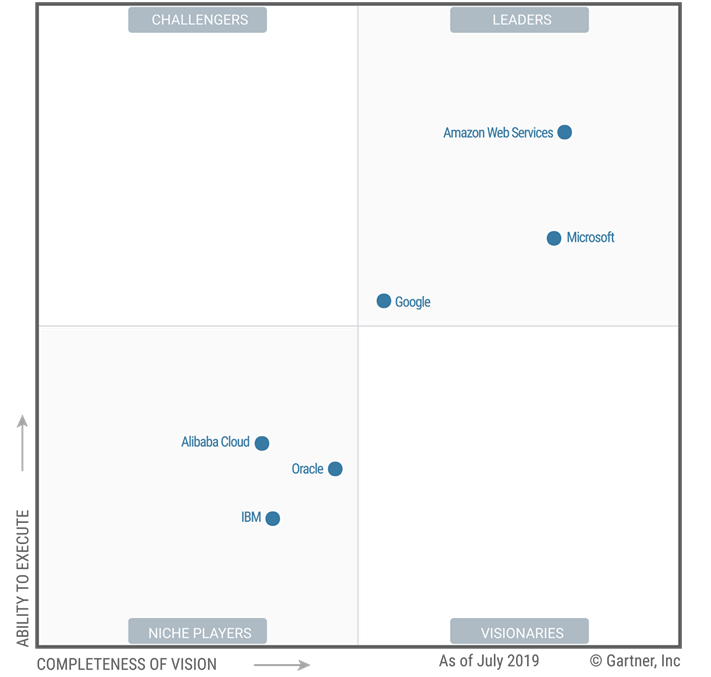
\includegraphics[width=0.9\textwidth]{figures/CloudIaaS.png}
\caption{Gartner (07/2019) pilvipalveluiden vertailu. \citep{top_cloud}}\label{gartner}
\end{figure}
